\documentclass[a4paper,12pt]{article}
\usepackage[utf8]{inputenc}
\usepackage[T1]{fontenc}
\usepackage{lmodern}
\usepackage{geometry}
\usepackage{setspace}
\usepackage{fancyhdr}
\usepackage{hyperref}
\usepackage{amsmath}
\usepackage{amsfonts}
\usepackage{amssymb}
\usepackage{mathtools}
\usepackage{float}
\usepackage{tabularx}
\usepackage{enumitem}
\usepackage{graphicx}
\usepackage{ragged2e}
\usepackage[spanish]{babel}
\usepackage{booktabs}
\usepackage{longtable}
\usepackage{multirow}
\usepackage{xcolor}
\usepackage{microtype}
\usepackage{caption}
\usepackage{textcomp}
\newcommand{\euro}{\texteuro}
\newcommand{\E}{\mathbb{E}}
\newcommand{\Var}{\mathrm{Var}}
\newcommand{\Cov}{\mathrm{Cov}}
\newcommand{\VaR}{\mathrm{VaR}}
\newcommand{\TVaR}{\mathrm{TVaR}}
\addto\captionsspanish{\renewcommand{\tablename}{Tabla}}
\addto\captionsspanish{\renewcommand{\figurename}{Figura}}
\captionsetup{font=small,labelfont=bf}

% Configuración de márgenes
\geometry{left=2.5cm,right=2.5cm,top=3cm,bottom=3cm}

% Configuración de encabezados y pies de página
\pagestyle{fancy}
\fancyhf{}
\renewcommand{\headrulewidth}{0pt}
\fancyfoot[C]{\thepage}

% Configuración de interlineado
\onehalfspacing
\justifying

% Configuración de hipervínculos
\hypersetup{
    hidelinks,
    colorlinks=false
}

\begin{document}

% Primera página (Título, Resumen y Abstract)
\begin{titlepage}
    \centering
    \vspace*{0.1cm}
    \huge\textbf{Tema 5: Preguntas de repaso}\\
    \vspace{1cm}
    \small{Luiz Alberto Luzuriaga Izquierdo}\\
    \vspace{0.1cm}
    Facultad de ciencias económicas, empresariales y turismo. \\
    \vspace{0.1cm}
    Universidad de Alcalá de Henares. \\
    \vspace{0.1cm}
    Curso 2026-2027\\
    \vspace{0.5cm}

{\bfseries Resumen}

\vspace{0.1cm}
\noindent
\begin{justify}
Respuestas razonadas a las tres preguntas de repaso del tema. Tema 5 (Teoría de valores extremos y riesgos catastróficos (POT / GPD)): Exceso sobre un umbral, distribución de Pareto generalizada, elección del umbral y paso de la severidad al capital anual.\\\\
\vspace{0.1cm}
\noindent
\textbf{Palabras clave}: valores extremos, GPD, umbral, riesgo catastrófico, preguntas de repaso.
\end{justify}
\begin{center}
    {\bfseries Abstract}
\end{center}
\vspace{0.1cm}
\noindent
\begin{justify}
Class work for Topic 5 of Actuarial Mathematics of Stability and Solvency of Insurance Activity: review questions with actuarial reasoning and numerical evidence.\\\\
\vspace{0.1cm}
\noindent
\textbf{Keywords}: extreme value theory, GPD, threshold, catastrophe risk, review questions.
\end{justify}

\end{titlepage}

% Índice
\newpage\pagenumbering{gobble}
\renewcommand{\contentsname}{Índice}
\newgeometry{left=4cm, right=4cm, top=3cm, bottom=2.5cm}
\tableofcontents

\restoregeometry
\newpage
\numberwithin{equation}{section}
\pagenumbering{arabic}
\setcounter{page}{1}

\section{Tema 5: Teoría de valores extremos y riesgos catastróficos (POT / GPD)}
\label{sec:tema5repaso}
\noindent
Respuestas razonadas a las tres preguntas de repaso del tema. Material de referencia: diapositivas del Tema 5 (Prof. Hugo González Riera).

\subsection{Pregunta 1 -- Fuentes de riesgo de modelo en un ajuste POT--GPD y su prueba de sensibilidad}

\noindent\textbf{Enunciado.} Identifica tres fuentes de riesgo de modelo en un ajuste POT--GPD (umbral, m\'etodo, estacionariedad, datos\dots) y prop\'on una prueba de sensibilidad para cada una.

\paragraph{Planteamiento.} Un cuantil extremo se obtiene por extrapolaci\'on: la GPD se ajusta a $N_u$ excesos y se usa mucho m\'as all\'a de los datos. Cada supuesto es una fuente de error. Se analizan seis; para cada una se da la prueba y el resultado en la muestra de la pr\'actica (2.000 siniestros Burr(2; 1,5; 5), $\xi=1/3$, $\VaR_{99,5}=27{,}85$ y $\TVaR_{99,5}=42{,}67$ M\euro, $T=40$ a\~nos).

\subsubsection*{1. El umbral $u$ (sesgo frente a varianza)}
Un $u$ bajo incluye excesos que no est\'an en el r\'egimen asint\'otico (sesgo); uno alto deja pocos datos (varianza). \textbf{Prueba:} reajustar con una rejilla de umbrales y examinar $\hat\xi(u)$, $\sigma^*(u)=\hat\sigma-\hat\xi u$ y los cuantiles, junto con el gr\'afico del exceso medio.
\begin{center}
\small
\begin{tabular}{rrrrrr}
\toprule
$u$ (M\euro) & $N_u$ & $\hat\xi$ & $\hat\sigma$ & $\VaR_{99,5}$ & $\TVaR_{99,5}$\\
\midrule
5 & 495 & 0,25 & 3,37 & 27,34 & 39,37\\
7,5 & 251 & 0,27 & 3,90 & 27,47 & 40,14\\
10 & 137 & 0,26 & 4,67 & 27,53 & 40,06\\
12,5 & 81 & 0,28 & 5,32 & 27,58 & 40,74\\
15 & 54 & 0,39 & 5,06 & 27,06 & 42,98\\
20 & 23 & 0,06 & 10,19 & 28,72 & 40,21\\
\bottomrule
\end{tabular}
\end{center}
El $\VaR_{99,5}$ es muy robusto (27,1--28,7; est\'a cerca de los datos); el $\TVaR$ depende de $\hat\xi$ (39--43). Por encima de $u\approx15$ hay menos de 55 excesos y $\hat\xi$ salta de 0,06 a 0,39. Se elige $u=10$ (primer umbral estable) y se reportan $u=7{,}5$ y $12{,}5$ como sensibilidad.

\subsubsection*{2. El m\'etodo de estimaci\'on}
\textbf{Prueba:} contrastar con m\'etodos de supuestos distintos (MLE, PWM/L-momentos, Hill, Pickands).
\begin{center}
\small
\begin{tabular}{lrr}
\toprule
M\'etodo & $\hat\xi$ & $\VaR_{99,5}$\\
\midrule
GPD--MLE ($u=10$) & 0,26 & 27,53\\
PWM / L-momentos & 0,26 & 27,45\\
Hill ($k=N_u=137$) & 0,41 & 29,17\\
Pickands ($k=34$) & 0,16 & --\\
Verdad & 0,33 & 27,85\\
\bottomrule
\end{tabular}
\end{center}
La dispersi\'on entre estimadores ($0{,}16$--$0{,}41$ alrededor del $0{,}33$ verdadero) es una medida honesta de la incertidumbre de la cola. Hill con $k$ grande est\'a sesgado al incluir cuerpo; Pickands tiene mucha varianza. Regla: no elegir el m\'etodo que da el n\'umero deseado.

\subsubsection*{3. La incertidumbre de los par\'ametros}
\textbf{Prueba:} intervalos de Wald (delta), de verosimilitud perfil y por \emph{bootstrap}. En $u=10$: $\hat\xi=0{,}26$, Wald $[0{,}05;0{,}47]$, perfil $[0{,}09;0{,}50]$, bootstrap $[0{,}01;0{,}47]$; $\VaR_{99,5}=27{,}5$ con Wald $[23{,}2;31{,}9]$; $\TVaR_{99,5}=40{,}1$ con bootstrap $[30{,}0;56{,}2]$. Los intervalos de perfil y bootstrap son asim\'etricos hacia la derecha.

\subsubsection*{4. La estacionariedad}
La EVT b\'asica supone excesos i.i.d. y frecuencia constante. \textbf{Prueba:} modelo $N_t\sim\text{Poisson}(\lambda(t))$, $\ln\lambda(t)=\beta_0+\beta_1(t-t_0)$ y contraste de raz\'on de verosimilitudes frente a $\beta_1=0$. En una simulaci\'on con 40 a\~nos y tendencia del $\approx25\%$ por d\'ecada: $\hat\beta_1=0{,}025$ (EE $0{,}009$), $LR=7{,}47$, $p=0{,}006$; el $\lambda$ actual es $3{,}62$ y suponer estacionariedad dar\'ia $2{,}25$ ($-38\%$); niveles de retorno a 100 y 200 a\~nos: $51{,}0$ y $62{,}7$ frente a $58{,}8$ y $72{,}0$ (Caso~2, $\xi=0{,}25$, $\sigma=4$, $u=5$).

\subsubsection*{5. Los datos: inflaci\'on, exposici\'on, franquicias, l\'imites y desarrollo}
Si no se homogeneizan, la GPD ajusta la historia de la cartera y no su riesgo actual. \textbf{Prueba:} reajustar bajo supuestos distintos de tratamiento (con y sin indexaci\'on; con y sin censura). Ejemplo con l\'imites de p\'oliza de 30 M\euro: 7 siniestros quedan topados. Ignorar la censura da $\hat\xi=0{,}02$ y $\VaR=24{,}63$ ($-10{,}5\%$ respecto al de los datos completos); la verosimilitud censurada $\sum\ln g(y_i)+\sum\ln[1-G(c_j)]$ da $\hat\xi=0{,}24$ y $\VaR=27{,}11$, casi el valor sin l\'imites ($0{,}26$ y $27{,}53$). Las franquicias exigen $u\ge d$ o verosimilitud truncada $f(x)/S(d)$; los siniestros abiertos deben proyectarse a coste \'ultimo.

\subsubsection*{6. La dependencia (agrupamiento) y la frecuencia}
Las reclamaciones de un mismo terremoto o tormenta no son independientes. \textbf{Prueba:} cambiar la cl\'ausula horaria (72/168 h) y el criterio de \emph{declustering}; comprobar el \'indice extremal $\theta$: ignorar $\theta<1$ infla $N_u$ y subestima los errores est\'andar de $\hat\xi$ (en un factor $\approx1/\sqrt\theta$). Para la frecuencia: Poisson frente a Binomial Negativa. Con $\Var(N)=2{,}5\,\E(N)$ el SCR simulado sube de $147$ a $216$ M\euro\ ($+47\%$) sin cambiar la GPD.

\paragraph{Ejemplo de la importancia relativa.} Un error de $\pm0{,}07$ en $\hat\xi$ mueve el SCR anual del Caso~1 entre $122$ y $177$ M\euro\ ($-17\%/+20\%$ sobre $147$); es mayor que muchos otros errores, de ah\'i que cada paso deba dejar evidencia documentada.

\bigskip\hrule\bigskip

\subsection{Pregunta 2 -- GEV (m\'aximos por bloques) frente a POT/GPD}

\noindent\textbf{Enunciado.} ?`Qu\'e diferencia hay entre el enfoque de m\'aximos por bloques (GEV) y el de excesos sobre un umbral (POT/GPD)? ?`Cu\'al usar\'ias para dimensionar el reaseguro anual de una cartera catastr\'ofica y por qu\'e?

\subsubsection*{Diferencias}
\begin{center}
\small
\begin{tabular}{p{3.2cm}p{5.8cm}p{5.8cm}}
\toprule
 & M\'aximos por bloques (GEV) & Excesos sobre umbral (POT/GPD)\\
\midrule
Resultado l\'imite & Fisher--Tippett--Gnedenko: $M_n$ normalizado $\to H_\xi$ & Balkema--Pickands--de Haan: excesos $\to$ GPD\\
Datos usados & el m\'aximo de cada bloque (p.~ej. a\~no) & todos los datos por encima de $u$\\
Eficiencia & baja: un dato por bloque (30--40 con 30--40 a\~nos) & mayor: aprovecha todos los extremos si son independientes\\
Elecci\'on clave & tama\~no del bloque & umbral $u$\\
Hace falta & m\'aximos o datos agregados & pérdidas por evento fechadas y homogeneizadas\\
Dependencia & el bloque la absorbe (agrupamiento intra-anual) & exige \emph{declustering}\\
\bottomrule
\end{tabular}
\end{center}
Ambos estiman la misma cola, con el mismo $\xi$.

\subsubsection*{El v\'inculo exacto}
Si los eventos que superan $u$ llegan como Poisson($\lambda_u$) con severidad GPD($\xi,\sigma$), el m\'aximo anual cumple
\[
P(M\le x)=\exp\Big\{-\lambda_u\big[1+\xi(x-u)/\sigma\big]^{-1/\xi}\Big\},
\]
que es exactamente una GEV con el \emph{mismo} $\xi$, localizaci\'on $\mu=u+\sigma(\lambda_u^{\xi}-1)/\xi$ y escala $\sigma_G=\sigma\lambda_u^{\xi}$. Con el Caso~1 ($\lambda_u=2$, $\xi=0{,}35$, $\sigma=6$): $\mu=14{,}71$, $\sigma_G=7{,}65$. El nivel 1-en-200 por la GEV, $132{,}31$, coincide con el del POT, $132{,}43$ (la peque\~na diferencia es $-\ln(1-1/200)$ frente a $1/200$); a 10, 50 y 100 a\~nos: POT $41{,}8$, $78{,}8$, $102{,}4$; GEV $40{,}9$, $78{,}5$, $102{,}2$.

\subsubsection*{Cu\'ando cada uno}
\textbf{POT} cuando hay p\'erdidas por evento fechadas y homogeneizadas, varios extremos por a\~no y la m\'etrica es por evento (Cat XL por evento, curva OEP, precio de capas). \textbf{GEV} cuando solo hay m\'aximos anuales (caudales, p\'erdida m\'axima anual), la unidad relevante es el a\~no o el agrupamiento intra-anual es fuerte y dif\'icil de depurar. La elecci\'on depende de los datos y de la unidad del contrato, no de que una teor\'ia sea mejor.

\subsubsection*{Para dimensionar el reaseguro anual de una cartera catastr\'ofica: POT con frecuencia y simulaci\'on}
\begin{enumerate}[leftmargin=*,itemsep=2pt]
\item Los contratos de reaseguro de cat\'astrofe se definen \emph{por evento} (Cat XL, cl\'ausula horaria 72/168 h): la GPD de la severidad por evento es la unidad natural, y las capas se tarifican con $E[(X-d)^+\mid X>u]$ y $\lambda_u$.
\item El POT usa todos los eventos grandes (137 en lugar de 40 m\'aximos anuales): intervalos m\'as estrechos. Con $N_u=30$ frente a $80$ el error t\'ipico de $\hat\xi$ pasa de $0{,}16$ a $0{,}29$.
\item Pero el capital y el reaseguro agregado son \emph{anuales}: se simula $N\sim$ Poisson($\lambda_u$) o Binomial Negativa, $X_i\sim$ GPD, se aplica el programa evento a evento y se obtienen las distribuciones OEP (m\'aximo) y AEP (suma). Con $10^6$ a\~nos: $E(S)=38{,}5$, $\VaR_{99,5}=185$, SCR $=147$ M\euro; OEP 1/200 $=132$ M\euro; con Binomial Negativa SCR $=216$.
\item La GEV complementa: sirve para contrastar la OEP anual y cuando solo existen m\'aximos.
\end{enumerate}

\paragraph{Conclusi\'on.} Para el reaseguro anual: POT (por evento, con $\lambda_u$ y declustering) y simulaci\'on anual; GEV como contraste o si faltan datos por evento.

\bigskip\hrule\bigskip

\subsection{Pregunta 3 -- $\hat\xi=0{,}6$: ?`qu\'e pasa con la varianza muestral?}

\noindent\textbf{Enunciado.} Si el ajuste arroja $\hat\xi=0{,}6$, ?`qu\'e implicaciones tiene sobre la fiabilidad de la varianza muestral de los grandes siniestros y qu\'e deber\'ias hacer?

\subsubsection*{Qu\'e momentos existen}
Con $\xi=0{,}6$ el \'indice de cola es $\alpha=1/\xi=1{,}67$. En la GPD, $\E[Y^k]<\infty$ solo si $k\xi<1$:
\begin{itemize}[leftmargin=*,itemsep=1pt]
\item $\E[Y]=\sigma/(1-\xi)=2{,}5\,\sigma$ \textbf{existe} ($\xi<1$);
\item $\Var(Y)=\infty$ pues $\xi>1/2$ (la condici\'on es $\xi<1/2$);
\item el tercer momento ($\xi<1/3$) tampoco existe.
\end{itemize}

\paragraph{V\'inculo con la Pareto (nota de clase).} Para $\xi>0$ la GPD es exactamente una Pareto reparametrizada: $\xi=1/\alpha$ y $\sigma(u)=(\theta+u)/\alpha$. Por eso las condiciones de existencia de momentos son las de la Pareto del modelo colectivo ($\alpha=1{,}67<2$: sin varianza), y $\hat\xi=0{,}6$ equivale al mismo diagn\'ostico que una Pareto con $\alpha\approx1{,}7$.

\subsubsection*{Por qu\'e la varianza muestral no es fiable}
Si la varianza poblacional es infinita, $s^2$ no converge a ning\'un valor: crece con el tama\~no de muestra y est\'a dominada por la mayor observaci\'on. Simulaci\'on con una GPD($\xi=0{,}6$, $\sigma=1$), 150 r\'eplicas por tama\~no:
\begin{center}
\small
\begin{tabular}{rrrr}
\toprule
$n$ & mediana de $s^2$ & percentil 90 & m\'aximo\\
\midrule
100 & 19 & 137 & 1.508\\
1.000 & 52 & 256 & 456.768\\
10.000 & 98 & 263 & 7.824\\
100.000 & 156 & 686 & 12.702\\
\bottomrule
\end{tabular}
\end{center}
La mediana de $s^2$ se multiplica por $8$ al pasar de $n=100$ a $n=10^5$ y la dispersi\'on entre muestras es enorme (a veces de varios \'ordenes de magnitud: con $n=1.000$ el m\'aximo observado fue 456.768 frente a una mediana de 52). El teorema central del l\'imite no se aplica: la media muestral converge a una ley estable de \'indice $1{,}67$ y lo hace lentamente (con $n=1.000$, su desviaci\'on t\'ipica es $0{,}46$ para una media de $2{,}5$, un $18\%$).
\begin{figure}[H]\centering
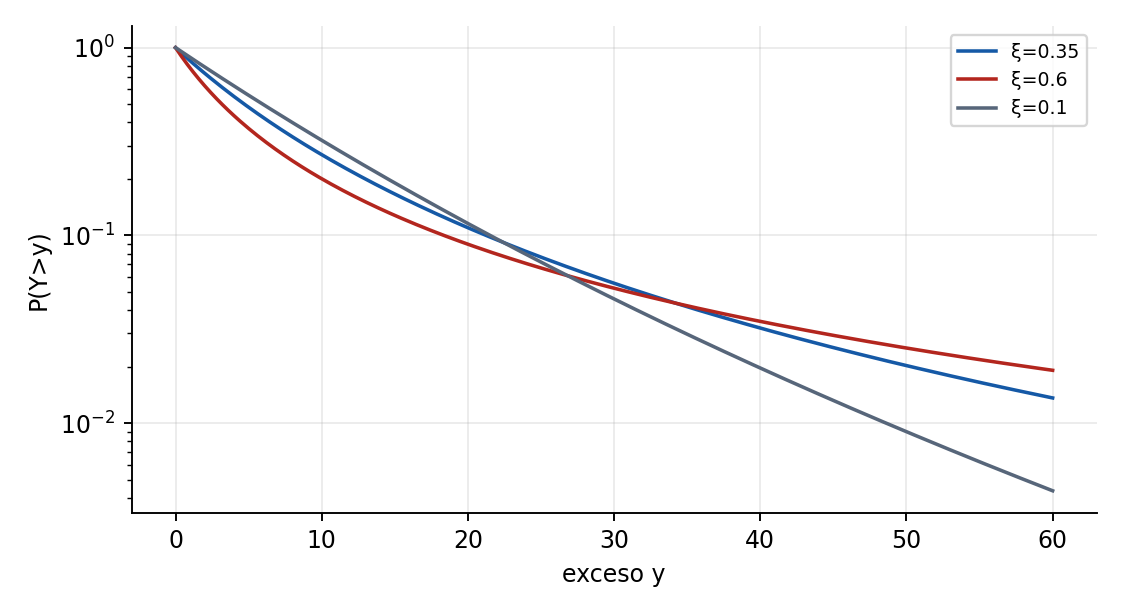
\includegraphics[width=.7\linewidth]{t5_f_repaso3.png}
\caption{Supervivencia de excesos de una GPD con la misma media y distinto $\xi$: con $\xi=0{,}6$ la cola es mucho m\'as pesada.}
\end{figure}

\subsubsection*{Qu\'e hacer}
\begin{enumerate}[leftmargin=*,itemsep=2pt]
\item \textbf{No usar medidas basadas en la varianza}: ni desviaci\'on t\'ipica, ni Normal/Normal Power, ni coeficientes de variaci\'on ni principios de prima por varianza (infinitos). Usar cuantiles, \emph{TVaR} (existe, $\xi<1$) y primas por capas.
\item \textbf{Cuantiles y TVaR del modelo GPD}: $\VaR_p=u+\frac\sigma\xi[r^{-\xi}-1]$ y $\TVaR_p=(\VaR_p+\sigma-\xi u)/(1-\xi)$; el cociente $\TVaR/\VaR\to1/(1-\xi)=2{,}5$ (frente a $1{,}54$ con $\xi=0{,}35$): el TVaR es dos veces y media el VaR.
\item \textbf{Cuantificar la incertidumbre de $\hat\xi$} (perfil, bootstrap): $SE(\hat\xi)\approx(1+\xi)/\sqrt{N_u}$; con $N_u=80$, $\pm0{,}18$ al 68\,\%; el intervalo puede incluir $\xi\ge1$ (media infinita) y entonces el TVaR no existe. Contrastar con Hill, PWM y diagn\'osticos.
\item \textbf{Acotar la cola con reaseguro de exceso de p\'erdida y l\'imites de p\'oliza}, de modo que la severidad retenida tenga momentos; y tratar $\xi\ge0{,}5$ como alerta.
\item Revisar que $\hat\xi=0{,}6$ no sea un artefacto: umbral demasiado bajo o alto, datos sin homogeneizar, mezcla de fen\'omenos (terremoto + incendio), pocas observaciones.
\end{enumerate}

\paragraph{Conclusi\'on.} Con $\xi\ge0{,}5$ la varianza deja de ser una magnitud con sentido; el riesgo debe medirse por cuantiles y por la cola con su intervalo de confianza, y gestionarse con reaseguro.

\subsubsection*{Referencias}
\begin{itemize}[leftmargin=*,itemsep=0pt]
\item Balkema, A. A. y de Haan, L. (1974). Residual life time at great age. \emph{The Annals of Probability}, 2(5).
\item Pickands, J. (1975). Statistical inference using extreme order statistics. \emph{The Annals of Statistics}, 3(1).
\item Embrechts, P., Kl\"uppelberg, C. y Mikosch, T. (1997). \emph{Modelling Extremal Events for Insurance and Finance}. Springer.
\item Coles, S. (2001). \emph{An Introduction to Statistical Modeling of Extreme Values}. Springer.
\item McNeil, A. J., Frey, R. y Embrechts, P. \emph{Quantitative Risk Management}. Princeton University Press.
\item Hosking, J. R. M. y Wallis, J. R. (1987). Parameter and quantile estimation for the generalized Pareto distribution. \emph{Technometrics}, 29(3).
\end{itemize}

\end{document}
